% Options for packages loaded elsewhere
\PassOptionsToPackage{unicode}{hyperref}
\PassOptionsToPackage{hyphens}{url}
%
\documentclass[
]{book}
\usepackage{lmodern}
\usepackage{amssymb,amsmath}
\usepackage{ifxetex,ifluatex}
\ifnum 0\ifxetex 1\fi\ifluatex 1\fi=0 % if pdftex
  \usepackage[T1]{fontenc}
  \usepackage[utf8]{inputenc}
  \usepackage{textcomp} % provide euro and other symbols
\else % if luatex or xetex
  \usepackage{unicode-math}
  \defaultfontfeatures{Scale=MatchLowercase}
  \defaultfontfeatures[\rmfamily]{Ligatures=TeX,Scale=1}
\fi
% Use upquote if available, for straight quotes in verbatim environments
\IfFileExists{upquote.sty}{\usepackage{upquote}}{}
\IfFileExists{microtype.sty}{% use microtype if available
  \usepackage[]{microtype}
  \UseMicrotypeSet[protrusion]{basicmath} % disable protrusion for tt fonts
}{}
\makeatletter
\@ifundefined{KOMAClassName}{% if non-KOMA class
  \IfFileExists{parskip.sty}{%
    \usepackage{parskip}
  }{% else
    \setlength{\parindent}{0pt}
    \setlength{\parskip}{6pt plus 2pt minus 1pt}}
}{% if KOMA class
  \KOMAoptions{parskip=half}}
\makeatother
\usepackage{xcolor}
\IfFileExists{xurl.sty}{\usepackage{xurl}}{} % add URL line breaks if available
\IfFileExists{bookmark.sty}{\usepackage{bookmark}}{\usepackage{hyperref}}
\hypersetup{
  pdftitle={Biostatistika Inferensial},
  pdfauthor={dimas \& ulya},
  hidelinks,
  pdfcreator={LaTeX via pandoc}}
\urlstyle{same} % disable monospaced font for URLs
\usepackage{color}
\usepackage{fancyvrb}
\newcommand{\VerbBar}{|}
\newcommand{\VERB}{\Verb[commandchars=\\\{\}]}
\DefineVerbatimEnvironment{Highlighting}{Verbatim}{commandchars=\\\{\}}
% Add ',fontsize=\small' for more characters per line
\usepackage{framed}
\definecolor{shadecolor}{RGB}{248,248,248}
\newenvironment{Shaded}{\begin{snugshade}}{\end{snugshade}}
\newcommand{\AlertTok}[1]{\textcolor[rgb]{0.94,0.16,0.16}{#1}}
\newcommand{\AnnotationTok}[1]{\textcolor[rgb]{0.56,0.35,0.01}{\textbf{\textit{#1}}}}
\newcommand{\AttributeTok}[1]{\textcolor[rgb]{0.77,0.63,0.00}{#1}}
\newcommand{\BaseNTok}[1]{\textcolor[rgb]{0.00,0.00,0.81}{#1}}
\newcommand{\BuiltInTok}[1]{#1}
\newcommand{\CharTok}[1]{\textcolor[rgb]{0.31,0.60,0.02}{#1}}
\newcommand{\CommentTok}[1]{\textcolor[rgb]{0.56,0.35,0.01}{\textit{#1}}}
\newcommand{\CommentVarTok}[1]{\textcolor[rgb]{0.56,0.35,0.01}{\textbf{\textit{#1}}}}
\newcommand{\ConstantTok}[1]{\textcolor[rgb]{0.00,0.00,0.00}{#1}}
\newcommand{\ControlFlowTok}[1]{\textcolor[rgb]{0.13,0.29,0.53}{\textbf{#1}}}
\newcommand{\DataTypeTok}[1]{\textcolor[rgb]{0.13,0.29,0.53}{#1}}
\newcommand{\DecValTok}[1]{\textcolor[rgb]{0.00,0.00,0.81}{#1}}
\newcommand{\DocumentationTok}[1]{\textcolor[rgb]{0.56,0.35,0.01}{\textbf{\textit{#1}}}}
\newcommand{\ErrorTok}[1]{\textcolor[rgb]{0.64,0.00,0.00}{\textbf{#1}}}
\newcommand{\ExtensionTok}[1]{#1}
\newcommand{\FloatTok}[1]{\textcolor[rgb]{0.00,0.00,0.81}{#1}}
\newcommand{\FunctionTok}[1]{\textcolor[rgb]{0.00,0.00,0.00}{#1}}
\newcommand{\ImportTok}[1]{#1}
\newcommand{\InformationTok}[1]{\textcolor[rgb]{0.56,0.35,0.01}{\textbf{\textit{#1}}}}
\newcommand{\KeywordTok}[1]{\textcolor[rgb]{0.13,0.29,0.53}{\textbf{#1}}}
\newcommand{\NormalTok}[1]{#1}
\newcommand{\OperatorTok}[1]{\textcolor[rgb]{0.81,0.36,0.00}{\textbf{#1}}}
\newcommand{\OtherTok}[1]{\textcolor[rgb]{0.56,0.35,0.01}{#1}}
\newcommand{\PreprocessorTok}[1]{\textcolor[rgb]{0.56,0.35,0.01}{\textit{#1}}}
\newcommand{\RegionMarkerTok}[1]{#1}
\newcommand{\SpecialCharTok}[1]{\textcolor[rgb]{0.00,0.00,0.00}{#1}}
\newcommand{\SpecialStringTok}[1]{\textcolor[rgb]{0.31,0.60,0.02}{#1}}
\newcommand{\StringTok}[1]{\textcolor[rgb]{0.31,0.60,0.02}{#1}}
\newcommand{\VariableTok}[1]{\textcolor[rgb]{0.00,0.00,0.00}{#1}}
\newcommand{\VerbatimStringTok}[1]{\textcolor[rgb]{0.31,0.60,0.02}{#1}}
\newcommand{\WarningTok}[1]{\textcolor[rgb]{0.56,0.35,0.01}{\textbf{\textit{#1}}}}
\usepackage{longtable,booktabs}
% Correct order of tables after \paragraph or \subparagraph
\usepackage{etoolbox}
\makeatletter
\patchcmd\longtable{\par}{\if@noskipsec\mbox{}\fi\par}{}{}
\makeatother
% Allow footnotes in longtable head/foot
\IfFileExists{footnotehyper.sty}{\usepackage{footnotehyper}}{\usepackage{footnote}}
\makesavenoteenv{longtable}
\usepackage{graphicx,grffile}
\makeatletter
\def\maxwidth{\ifdim\Gin@nat@width>\linewidth\linewidth\else\Gin@nat@width\fi}
\def\maxheight{\ifdim\Gin@nat@height>\textheight\textheight\else\Gin@nat@height\fi}
\makeatother
% Scale images if necessary, so that they will not overflow the page
% margins by default, and it is still possible to overwrite the defaults
% using explicit options in \includegraphics[width, height, ...]{}
\setkeys{Gin}{width=\maxwidth,height=\maxheight,keepaspectratio}
% Set default figure placement to htbp
\makeatletter
\def\fps@figure{htbp}
\makeatother
\setlength{\emergencystretch}{3em} % prevent overfull lines
\providecommand{\tightlist}{%
  \setlength{\itemsep}{0pt}\setlength{\parskip}{0pt}}
\setcounter{secnumdepth}{5}
\usepackage{booktabs}
\usepackage{amsthm}
\makeatletter
\def\thm@space@setup{%
  \thm@preskip=8pt plus 2pt minus 4pt
  \thm@postskip=\thm@preskip
}
\makeatother
\usepackage[]{natbib}
\bibliographystyle{apalike}

\title{Biostatistika Inferensial}
\author{dimas \& ulya}
\date{2021-01-26}

\begin{document}
\maketitle

{
\setcounter{tocdepth}{1}
\tableofcontents
}
\hypertarget{pengantar}{%
\chapter{Pengantar}\label{pengantar}}

Modul ini dibuat sebagai bahan ajar pada mata kuliah Biostatistika Inferensial Fakultas Kesehatan Masyarakat Universitas Jember. Pada buku ini akan membahas beberapa topik perkuliahan yaitu:

\begin{itemize}
\tightlist
\item
  Uji 2 sampel independen
\item
  Uji 2 sampel berpasangan
\item
  Uji Anova
\item
  Uji Korelasi
\item
  Uji Regresi Linier
\end{itemize}

\hypertarget{uji2sampelind}{%
\chapter{Uji 2 Sampel Independen}\label{uji2sampelind}}

\hypertarget{tujuan}{%
\section{Tujuan}\label{tujuan}}

\begin{itemize}
\tightlist
\item
  Mahasiswa mampu memahami konsep dasar pengujian 2 sampel independen
\item
  Mahasiswa mampu melakukan melakukan pengujian 2 sampel independen secara manual
\item
  Mahasiswa mampu melakukan melakukan pengujian 2 sampel independen menggunakan aplikasi pengolah data
\end{itemize}

\hypertarget{dasar-teori}{%
\section{Dasar Teori}\label{dasar-teori}}

Terkadang kita ingin mengetahui apakah sebuah kelompok data (sampel data) memiliki nilai rata-rata yang sama dengan kelompok data yang lain. Tentu kata ``sama'' dalam hal ini tidak memiliki arti sama persis sebab hal ini sangat jarang terjadi. Akan selalu ada kesalahan yang dapat ditolernasi di setiap pengujian.

Andaikan dari 10 sampel mahasiswa laki-laki diperoleh rata-rata tinggi badan = 168,5 dan dari 10 sampel mahasiswa perempuan diperoleh tinggi badan = 167,2. Apakah dapat disimpulkan bahwa tinggi badan mahasiswa laki-laki = tinggi badan mahasiswa perempuan? Jika ``ya'', maka apa dasar pengambilan kesimpulan tersebut?

Uji 2 sampel independen merupakan uji statistik yang digunakan untuk menguji nilai rata-rata dari 2 kelompok/sampel/populasi yang saling bebas. Terdapat 2 pengujian yang dapat dilakukan pada kasus ini, yang pertama adalah Uji t 2 Sampel Independen (parametrik) dan Uji Mann Whitney (non-parametrik).

Berikut ini adalah contoh kasus 2 sampel independen (yang saling bebas):

\begin{itemize}
\tightlist
\item
  Kepala Dinas Kesehatan ingin menguji apakah ada perbedaan jumlah kunjungan pada puskesmas yang berada di daerah perkotaan dan daerah pedesaan.
\item
  Seorang peneliti menduga bahwa terdapat perbedaan kandungan gizi antara roti tawar yang biasa dengan roti tawar yang telah ditambahkan dengan tepung kelor.
\item
  Perusahaan farmasi A meyakini bahwa produk obat penurun gula darah yang mereka produksi dapat menurunkan kadar gula lebih baik daripada produk dari perusahaan farmasi B
\end{itemize}

\hypertarget{hipotesis-pengujian}{%
\subsection{Hipotesis Pengujian}\label{hipotesis-pengujian}}

Terdapat 3 hipotesis yang dapat digunakan dalam melakukan pengujian dengan menggunakan Uji t 2 Sampel Independen.

\textbf{Hipotesis Satu Arah Kanan}\\
Hipotesis ini digunakan untuk menguji apakah rata-rata dari suatu sampel/kelompok lebih besar dari sampel/kelompok yang lain. Hipotesis ditulis sebagai berikut:\\
\(H_0 : \mu_1-\mu_2 \leq d_0\)\\
\(H_1 : \mu_1-\mu_2 > d_0\)

Apabila \(d_0 = 0\), maka hipotesis akan menjadi:\\
\(H_0 : \mu_1 \leq \mu_2\)\\
\(H_1 : \mu_1 > \mu_2\)

Daerah penolakan dan penerimaan \(H_0\) pada \(\alpha = 5\%\) dan \(df = 10000\) dapat dilihat pada gambar berikut:

\begin{center}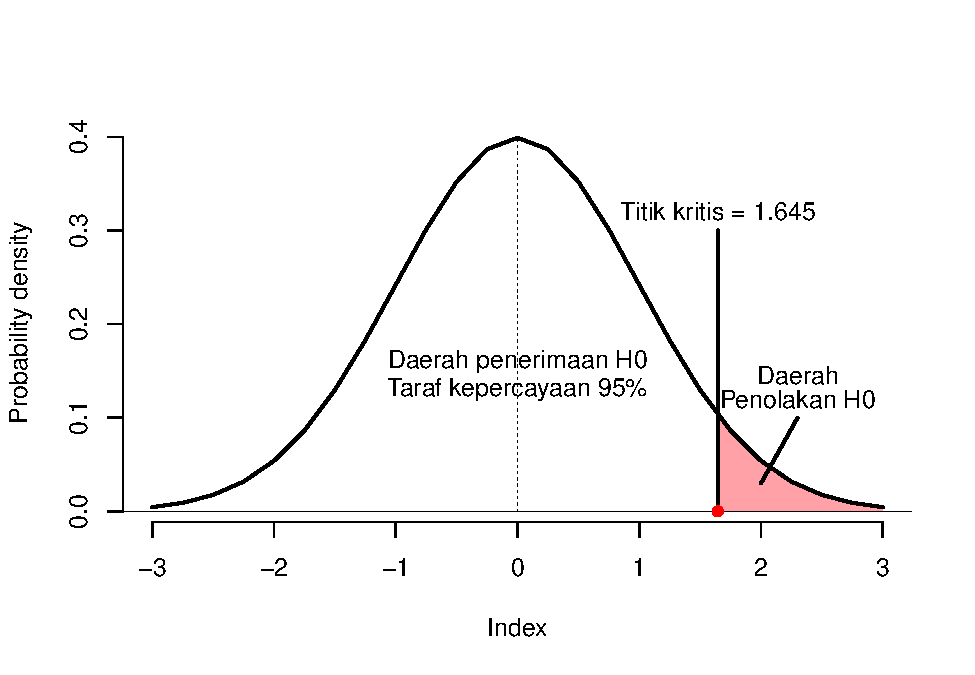
\includegraphics[width=0.75\linewidth,height=0.75\textheight]{bookdown-demo_files/figure-latex/unnamed-chunk-2-1} \end{center}

Penolakan \(H_0\) dilakukan apabila nilai \(t_{hitung}\) berada pada daerah penolakan H0 (\(t_{hitung}\) \textgreater{} nilai kritis \(1.645\)).

\textbf{Hipotesis Satu Arah Kiri}\\
Hipotesis ini digunakan untuk menguji apakah rata-rata dari suatu sampel/kelompok lebih kecil dari sampel/kelompok yang lain. Hipotesis ditulis sebagai berikut:\\
\(H_0 : \mu_1-\mu_2 \geq d_0\)\\
\(H_1 : \mu_1-\mu_2 < d_0\)

Apabila \(d_0 = 0\), maka hipotesis akan menjadi:\\
\(H_0 : \mu_1 \geq \mu_2\)\\
\(H_1 : \mu_1 < \mu_2\)

Daerah penolakan dan penerimaan \(H_0\) pada \(\alpha = 5\%\) dan \(df = 10000\) dapat dilihat pada gambar berikut:

\begin{center}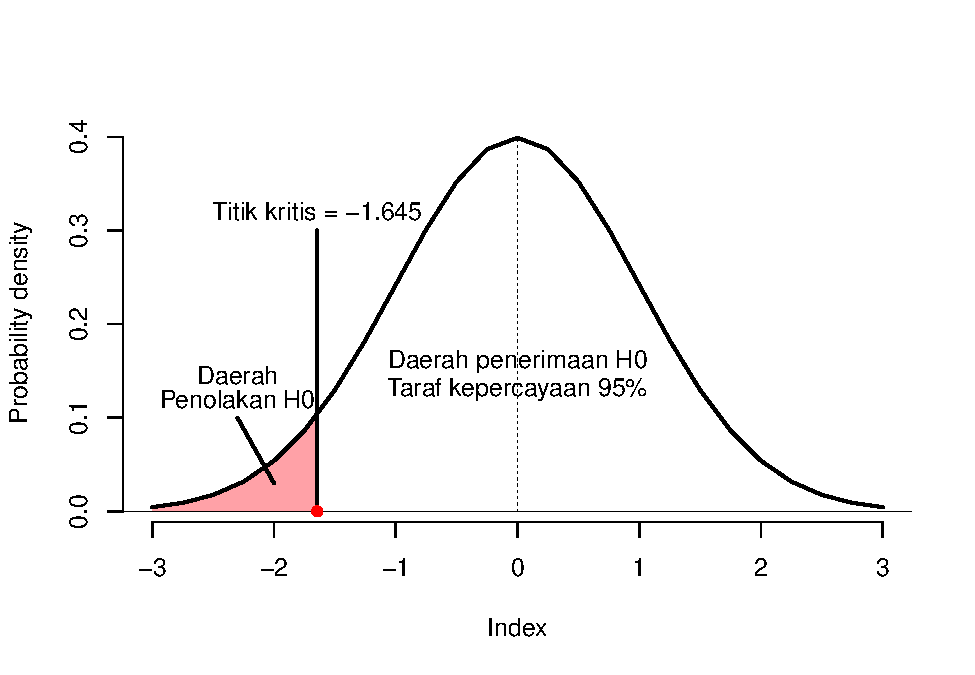
\includegraphics[width=0.75\linewidth,height=0.75\textheight]{bookdown-demo_files/figure-latex/unnamed-chunk-4-1} \end{center}

Penolakan \(H_0\) dilakukan apabila nilai \(t_{hitung}\) berada pada daerah penolakan H0 (\(t_{hitung}\) \textless{} nilai kritis \(-1.645\)).

\textbf{Hipotesis Dua Arah}\\
Hipotesis ini digunakan untuk menguji apakah rata-rata dari suatu sampel/kelompok berbeda (dapat lebih besar atau lebih kecil) dari sampel/kelompok yang lain. Hipotesis ditulis sebagai berikut:\\
\(H_0 : \mu_1-\mu_2 = d_0\)\\
\(H_1 : \mu_1-\mu_2 \neq d_0\)

Apabila \(d_0 = 0\), maka hipotesis akan menjadi:\\
\(H_0 : \mu_1 = \mu_2\)\\
\(H_1 : \mu_1 \neq \mu_2\)

Daerah penolakan dan penerimaan \(H_0\) pada \(\alpha = 5\%\) dan \(df = 10000\) dapat dilihat pada gambar berikut:

\begin{center}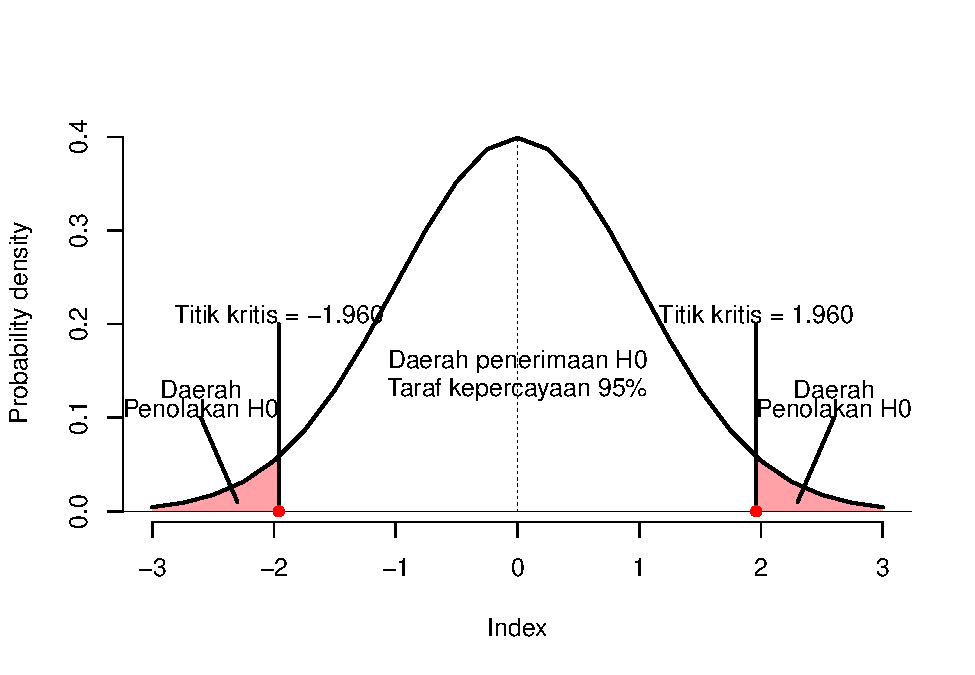
\includegraphics[width=0.75\linewidth,height=0.75\textheight]{bookdown-demo_files/figure-latex/unnamed-chunk-6-1} \end{center}

Penolakan \(H_0\) dilakukan apabila nilai \(t_{hitung}\) berada pada daerah penolakan H0 (\(t_{hitung}\) \textless{} nilai kritis \(-1.960\) bila \(t_{hitung}\) negatif atau \(t_{hitung}\) \textgreater{} nilai kritis \(1.960\) bila \(t_{hitung}\) positif).

\hypertarget{uji-t-2-sampel-independen}{%
\subsection{Uji t 2 Sampel Independen}\label{uji-t-2-sampel-independen}}

Uji t 2 Sampel Independen memiliki beberapa asumsi yang harus terpenuhi, yaitu:

\begin{itemize}
\tightlist
\item
  Sampel/kelompok diambil secara acak
\item
  Sampel/kelompok independen
\item
  Sampel/kelompok berasal dari populasi yang berdistribusi normal
\item
  Memiliki varians antar sampel/kelompok yang sama (homogen)
\end{itemize}

Namun pada kasus kedua sampel tidak memiliki varians yang sama (homogen), uji dapat dilanjutkan dengan menggunakan derajat kebebasan yang berbeda.

Formula untuk Uji t 2 Sampel Independen (\(t_{hitung}\)) dengan asumsi varians antar kelompok sama ialah sebagai berikut:
\[
t = \frac{(\bar{X_1}-\bar{X_2})-(\mu_1-\mu_2)}{\sqrt{\frac{\sigma_1^2}{n_1}+\frac{\sigma_2^2}{n_2}}}
\]
dimana:

\begin{itemize}
\tightlist
\item
  derajat kebebasan sama dengan \(n-1\) (pada kasus \(n_1\) dan \(n_2\) yang sama)
\item
  pada kasus varians populasi (\(\sigma^2\)) tidak diketahui maka \(\sigma^2 = s^2 = \frac{\sum(x_i-\mu)}{n-1}\).
\end{itemize}

Selain itu, \(t_{hitung}\) juga dapat dihitung dengan formula berikut:
\[
t = \frac{(\bar{X_1}-\bar{X_2})-(\mu_1-\mu_2)}{s_p\sqrt{\frac{1}{n_1}+\frac{1}{n_2}}}
\]
dimana \(s_p = \sqrt{\frac{(n_1-1)s^2_1+(n_2-1)s^2_2}{n_1+n_2-2}}\).

Apabila hasil pengujian varians dinyatakan bahwa kedua sampel/kelompok tidak memiliki varians yang sama (homogen), maka derajat kebebasan dihitung dengan formula berikut:
\[
d.f = \frac{(s_1^2/n_1+s_2^2/n_2)^2}{(s_1^2/n_1)^2/(n_1-1)+(s_2^2/n_2)^2/(n_2-1)}
\]

\hypertarget{contoh}{%
\subsubsection{Contoh}\label{contoh}}

Berikut adalah contoh-contoh pengujian dengan menggunakan Uji t 2 Sampel Independen

\hypertarget{kasus-1}{%
\paragraph{Kasus 1}\label{kasus-1}}

Diketahui bahwa dalam 8 kali percobaan, rata-rata Ani dapat mengetik sebanyak 105 kata dengan standar deviasi 7 kata dalam waktu 1 menit. Dengan jumlah percobaan yang sama dengan Ani, Rudi dapat mengetik dengan rata-rata 115 kata dengan standar deviasi 10 dalam waktu 1 menit. Dengan menggunakan \(\alpha\) sebesar 5\%, apakah dapat disimpulkan bahwa Rudi dapat mengetik lebih cepat daripada Ani? Varians antar kelompok diasumsikan homogen.

\textbf{Jawab}\\

\begin{table}

\caption{\label{tab:anru-tab}Statistik Anis dan Rudi}
\centering
\begin{tabular}[t]{ccc}
\toprule
Statistik & Ani & Rudi\\
\midrule
n & 8 & 8\\
rata-rata & 105 & 115\\
standar deviasi & 7 & 10\\
\bottomrule
\end{tabular}
\end{table}

\emph{Langkah-langkah pengerjaan}

\begin{enumerate}
\def\labelenumi{\arabic{enumi}.}
\tightlist
\item
  Tentukan hipotesis pengujian:\\
  \(H_0 : \mu_1 \geq \mu_2\)\\
  \(H_0 : \mu_1 < \mu_2\)\\
  dimana \(\mu_1\) adalah rata-rata mengetik Rudi (populasi) dan \(\mu_2\) adalah rata-rata mengetik Ani (populasi)
\item
  Hitung derajat kebebasan \(dk = n - 1 = 8 - 1 = 7\).
\item
  Tentukan nilai \(t_{tabel}\) dengan \(alpha=0.05\) dan \(dk = 7\), sehingga \(t_{(0.05,7)} = 1,8946\).
\item
  Hitung nilai \(t_{hitung}\) dengan menganggap bahwa \(\mu_1-\mu_2 = 0\), maka:\\
  \[
  t_{hitung} = \frac{(\bar{X_1}-\bar{X_2})}{\sqrt{\frac{s_1^2}{n_1}+\frac{s_2^2}{n_2}}}
  \]
  \[
  t_{hitung} = \frac{(115-105)}{\sqrt{\frac{10^2}{8}+\frac{7^2}{8}}} = 2,32
  \]
\item
  Bandingkan \(t_{hitung}\) dengan \(t_{tabel}\) (\(2,32 > 1,8946\)).
\item
  Pengambilan keputusan: Tolak \(H_0\) (karena \(t_{hitung}\) lebih besar dari \(t_{tabel}\)).
\end{enumerate}

Sehingga dapat disimpulkan bahwa dengan menggunakan \(alpha = 5\%\) Rudi mengetik lebih cepat daripada Ani.

\hypertarget{kasus-2}{%
\paragraph{Kasus 2}\label{kasus-2}}

\hypertarget{kasus-3}{%
\paragraph{Kasus 3}\label{kasus-3}}

\hypertarget{uji-mann-whitney}{%
\section{Uji Mann Whitney}\label{uji-mann-whitney}}

\hypertarget{uji-dengan-spss}{%
\section{Uji dengan SPSS}\label{uji-dengan-spss}}

You can label chapter and section titles using \texttt{\{\#label\}} after them, e.g., we can reference Chapter \ref{intro}. If you do not manually label them, there will be automatic labels anyway, e.g., Chapter \ref{methods}.

Figures and tables with captions will be placed in \texttt{figure} and \texttt{table} environments, respectively.

\begin{Shaded}
\begin{Highlighting}[]
\KeywordTok{par}\NormalTok{(}\DataTypeTok{mar =} \KeywordTok{c}\NormalTok{(}\DecValTok{4}\NormalTok{, }\DecValTok{4}\NormalTok{, }\FloatTok{.1}\NormalTok{, }\FloatTok{.1}\NormalTok{))}
\KeywordTok{plot}\NormalTok{(pressure, }\DataTypeTok{type =} \StringTok{'b'}\NormalTok{, }\DataTypeTok{pch =} \DecValTok{19}\NormalTok{)}
\end{Highlighting}
\end{Shaded}

\begin{figure}

{\centering 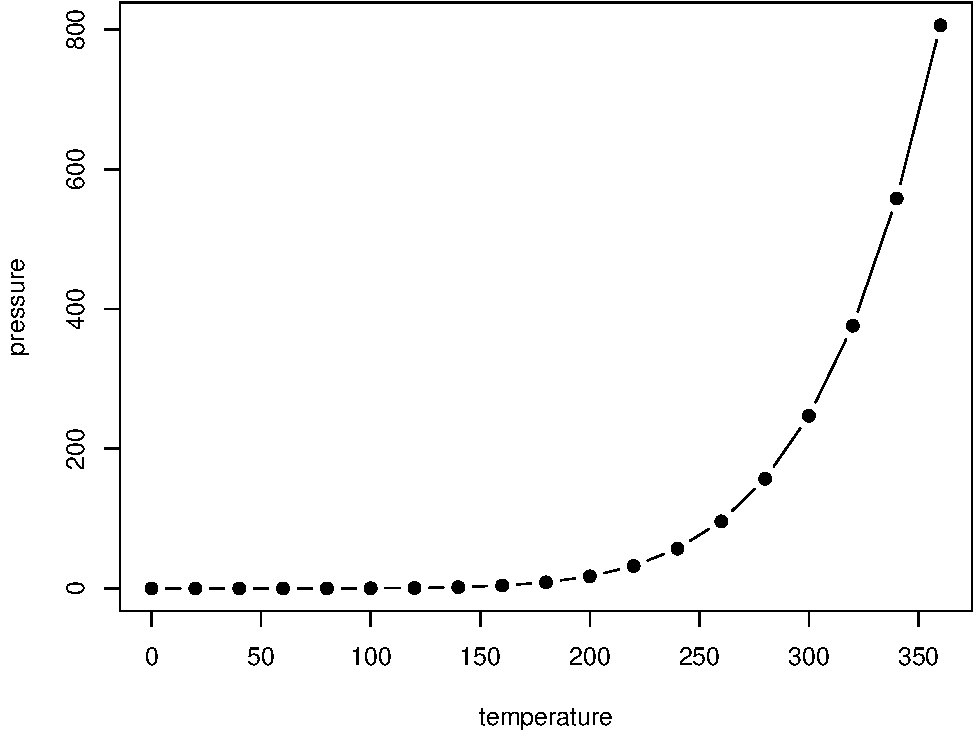
\includegraphics[width=0.8\linewidth]{bookdown-demo_files/figure-latex/nice-fig-1} 

}

\caption{Here is a nice figure!}\label{fig:nice-fig}
\end{figure}

Reference a figure by its code chunk label with the \texttt{fig:} prefix, e.g., see Figure \ref{fig:nice-fig}. Similarly, you can reference tables generated from \texttt{knitr::kable()}, e.g., see Table \ref{tab:nice-tab}.

\begin{Shaded}
\begin{Highlighting}[]
\NormalTok{knitr}\OperatorTok{::}\KeywordTok{kable}\NormalTok{(}
  \KeywordTok{head}\NormalTok{(iris, }\DecValTok{20}\NormalTok{), }\DataTypeTok{caption =} \StringTok{'Here is a nice table!'}\NormalTok{,}
  \DataTypeTok{booktabs =} \OtherTok{TRUE}
\NormalTok{)}
\end{Highlighting}
\end{Shaded}

\begin{table}

\caption{\label{tab:nice-tab}Here is a nice table!}
\centering
\begin{tabular}[t]{rrrrl}
\toprule
Sepal.Length & Sepal.Width & Petal.Length & Petal.Width & Species\\
\midrule
5.1 & 3.5 & 1.4 & 0.2 & setosa\\
4.9 & 3.0 & 1.4 & 0.2 & setosa\\
4.7 & 3.2 & 1.3 & 0.2 & setosa\\
4.6 & 3.1 & 1.5 & 0.2 & setosa\\
5.0 & 3.6 & 1.4 & 0.2 & setosa\\
\addlinespace
5.4 & 3.9 & 1.7 & 0.4 & setosa\\
4.6 & 3.4 & 1.4 & 0.3 & setosa\\
5.0 & 3.4 & 1.5 & 0.2 & setosa\\
4.4 & 2.9 & 1.4 & 0.2 & setosa\\
4.9 & 3.1 & 1.5 & 0.1 & setosa\\
\addlinespace
5.4 & 3.7 & 1.5 & 0.2 & setosa\\
4.8 & 3.4 & 1.6 & 0.2 & setosa\\
4.8 & 3.0 & 1.4 & 0.1 & setosa\\
4.3 & 3.0 & 1.1 & 0.1 & setosa\\
5.8 & 4.0 & 1.2 & 0.2 & setosa\\
\addlinespace
5.7 & 4.4 & 1.5 & 0.4 & setosa\\
5.4 & 3.9 & 1.3 & 0.4 & setosa\\
5.1 & 3.5 & 1.4 & 0.3 & setosa\\
5.7 & 3.8 & 1.7 & 0.3 & setosa\\
5.1 & 3.8 & 1.5 & 0.3 & setosa\\
\bottomrule
\end{tabular}
\end{table}

You can write citations, too. For example, we are using the \textbf{bookdown} package \citep{R-bookdown} in this sample book, which was built on top of R Markdown and \textbf{knitr} \citep{xie2015}.

\hypertarget{uji-2-sampel-berpasangan}{%
\chapter{Uji 2 Sampel Berpasangan}\label{uji-2-sampel-berpasangan}}

Here is a review of existing methods.

\hypertarget{uji-anova}{%
\chapter{Uji Anova}\label{uji-anova}}

We describe our methods in this chapter.

\hypertarget{uji-korelasi}{%
\chapter{Uji Korelasi}\label{uji-korelasi}}

Some \emph{significant} applications are demonstrated in this chapter.

\hypertarget{example-one}{%
\section{Example one}\label{example-one}}

\hypertarget{example-two}{%
\section{Example two}\label{example-two}}

\hypertarget{final-words}{%
\chapter{Final Words}\label{final-words}}

We have finished a nice book.

  \bibliography{book.bib,packages.bib}

\end{document}
